\large
Particles produced in the $pp$ collisions inside ATLAS can 
interact with the detector sub-systems
with each type of particle leaving a unique signature.
Reconstructing and identifying these particles precisely and efficienctly 
using the information recorded in each sub-detector is a 
building block of physics analysis.
Therefore, the following chapter outlines the reconstruction procedure of 
the particles important for the analysis present in this thesis.
\section{Track and vertex reconstruction}
\label{sec:track}
Track and vertex reconstruction is the starting point 
of physics objects reconstruction, 
which makes it crucial to understand how they are implemented in ATLAS.
Track reconstruction~\cite{ATLAS-CONF-2012-042,PERF-2015-08} is performed 
mainly with the so-called ``inside-outside'' procedure, 
complemented by the ``outside-in'' tracking and 
and the reconstruction of TRT-standalone tracks. 
% As shown in Figure~\ref{fig:electron_recon}, a charged particle traverses
% the ID. Space points are formed using the ID information.
The inside-out stage starts by assembling the raw measurements
into \textit{clusters}:
an algorithm called connected component analysis~\cite{CCA} 
groups pixels and strips in a given sensor, 
where the deposited energy yields a charge above threshold, 
with a common edge or corner into clusters. 
% It is useful to introduce the several classes of clusters identified 
% by either the ``truth information'' (TODO: remove if this is mentioned earlier in the simulation), 
% only available in simulation and referring to information at MC generator level, 
% or reconstructed quantities in both collision data and MC simulation. 
% Clusters created by charge deposits from one particle
% are called \textit{single-particle} clusters, and clusters created by charge
% deposits from multiple particles are called \textit{merged} clusters.
% These definitions rely on truth information and both cases
% are illustrated in Figure \ref{fig:cluster}. 
% In addition, clusters that are used in multiple reconstructed tracks 
% but are not sufficiently compatible with the properties of a merged cluster
% to be identified as merged by the reconstruction are called \textit{shared} clusters.
%  \begin{figure}[bth]
%     \centering
%     \begin{subfigure}[t]{.38\linewidth}
%         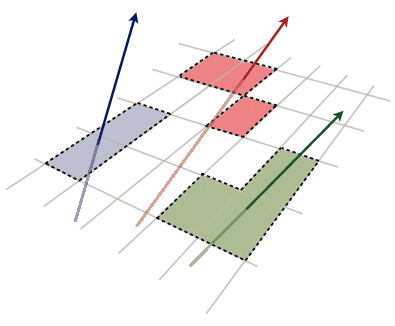
\includegraphics[width=1\textwidth]{Reconstruction/plots/single_cluster.png}
%         \caption{(a)}
%     \end{subfigure}
%     \begin{subfigure}[t]{.38\linewidth}
%         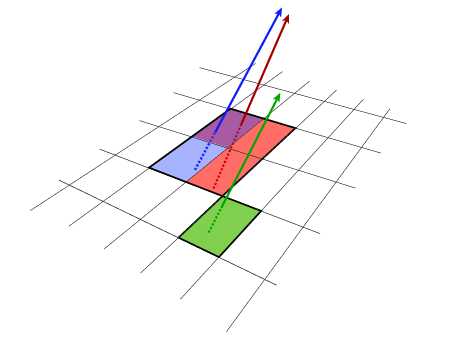
\includegraphics[width=1\textwidth]{Reconstruction/plots/merged_cluster.png}
%         \caption{(b)}
%     \end{subfigure}
    
%     \caption{Illustration of (a) single-particle pixel clusters on a pixel sensor and (b) 
%     a merged pixel cluster due to very collimated charged particles. 
%     Different colours represent energy deposits from different charged particles 
%     traversing the sensor and the particles trajectories are shown as arrows. 
%     Image taken from \cite{PERF-2015-08}.}
%     \label{fig:cluster}
% \end{figure}
From clusters, three-dimensional measurements, referred to as
\textit{space points}, are created (the yellow points in Figure~\ref{fig:track_recon}). 
They represent the point where the charged particle 
traversed the active material of the ID. 
Each space point equates to one cluster in the pixel detector, while in the SCT, 
clusters from both sides of a strip layer must be combined 
to obtain a three-dimensional measurement.
Three space points are combined to form track seeds 
(circled in blue in Figure~\ref{fig:track_recon}). 
% This approach maximizes the possible number of combinations while still allowing 
% a first crude momentum estimate. 
% The impact parameters of a track seed, 
% with respect to the centre of the interaction region, are estimated by assuming 
% a perfect helical trajectory in a uniform magnetic field.
A combinatorial Kalman filter~\cite{FRUHWIRTH1987444} is then used to 
build track candidates from the chosen seeds by incorporating additional 
space points from the remaining layers of the pixel and SCT detectors which 
are compatible with the preliminary trajectory 
(circled in a blue dashed line in Figure~\ref{fig:track_recon}). 
\begin{figure}[bht]
    \begin{centering}	
    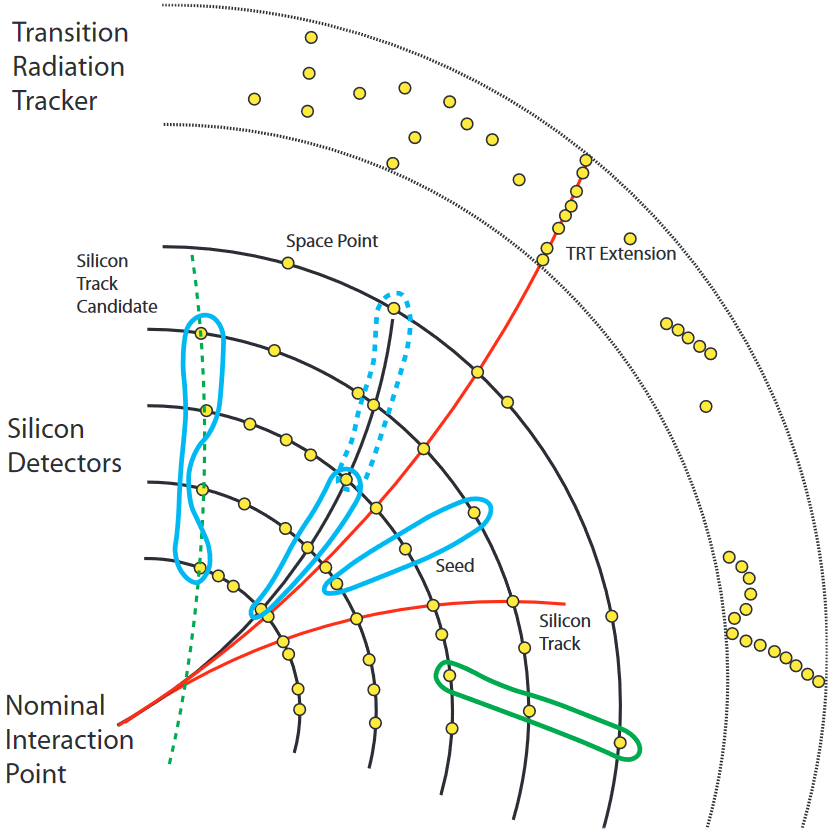
\includegraphics[width=.8\textwidth]{Reconstruction/plots/track.png}
    \caption{An example of track reconstruction. 
    Image reproduced from Ref.~\cite{ATLAS-CONF-2010-072}.
        }
    \label{fig:track_recon}
    \end{centering}
\end{figure}
A track score computed by the quantities of the fitted track
is assigned to each track.
% including the $\chi^2$ of the fitting, intrinsic resolution, 
% expected clusters multiplicity, number of holes (missing hits) 
% and \pt. 
The tracks candidates are processed in descending order of 
track score and those that fail 
a set of minimum requirements on \pt, the number of holes, 
and the number of clusters etc are rejected;
candidates that have too many bad quality clusters are 
stripped down and re-scored, then returned to the list
of remaining candidates.
This process is referred to as ``ambiguity solving''~\cite{PERF-2015-08}.
%  track candidates are fitted if they fulfil 
% a set of minimum requirement 
% on \pt\, number of holes, number of clusters etc.
% After that, the fitted tracks with too many shared clusters 
% (with additional artificial neural network to identify these shared clusters)  
% are striped down and re-scored, 
% and returned to the ordered list of remaining candidates;
% the fitted tracks with too many holes or too few clusters are rejected;
% those pass through the above requirement are accpeted and added 
% to the final track collection. 
% This process is referred to as ``ambiguity solving''~\cite{PERF-2015-08}.
Finally, the tracks are extended into the TRT and, by using the full information
of all three sub-detectors, the tracks are fitted again to determine the final track
parameters. The track can be fully represented 
by five parameters measured at the perigee,
which are the impact parameter 
(IP, transverse distance from the interaction point) $d_0$, 
the distance from the interaction point along the $z$ axis $z_0$,
the azimuthal angle $\phi$, the polar angle $\theta$ 
and the charge-momentum ratio $q/p_T$.

The complementary ``outside-in'' algorithm starts with searching for tracks with segments 
reconstructed in the TRT, and extend the tracks inwards by adding silicon hits.
The tracks are built with the combinatorial Kalman filter and passed to the
ambiguity solving procedure.
% Back-tracking is designed to reconstruct tracks of secondary particles, which are
% produced in the interactions of primary particles.
Finally, tracks with a TRT segment but no extension into the silicon detectors
are referred as TRT-standalone tracks. 

After the tracks are reconstructed, primary vertices,
which are the points where the hard-scattering processes occured,
are reconstructed in two steps~\cite{ATLAS-CONF-2010-069}:
a) the primary vertex finding algorithm, 
dedicated to associate reconstructed tracks to the vertex candidates, 
and b) the vertex fitting algorithm, 
dedicated to reconstruct the vertex position and 
its corresponding erorr matrix. 
It also refits the associated
tracks constraining them to originate 
from the reconstructed interaction point.
The vertex finding algorithm works as follows:
first, vertex seeds are obtained from the $z$-position 
at the beamline of the reconstructed tracks; 
and then, an iterative $\chi^2$ fit is then performed 
using the vertex seed and nearby tracks. 
% Each track carries a weight which is a measure of its compatibility 
% with the fitted vertex. 
Vertices are required to contain at least two tracks, and 
tracks displaced by more than 7$\sigma$ from the vertex are used to
seed a new vertex.  The procedure is repeated 
until no additional vertices can be found, 
and no unassociated tracks are left in the event.
The primary vertex for each event is selected as the vertex with the highest
$\sum_{tracks}(p_T^{track})^2$.


